\section{Introduction}

\begin{frame}{3D representations of urban spaces}
	\centering
	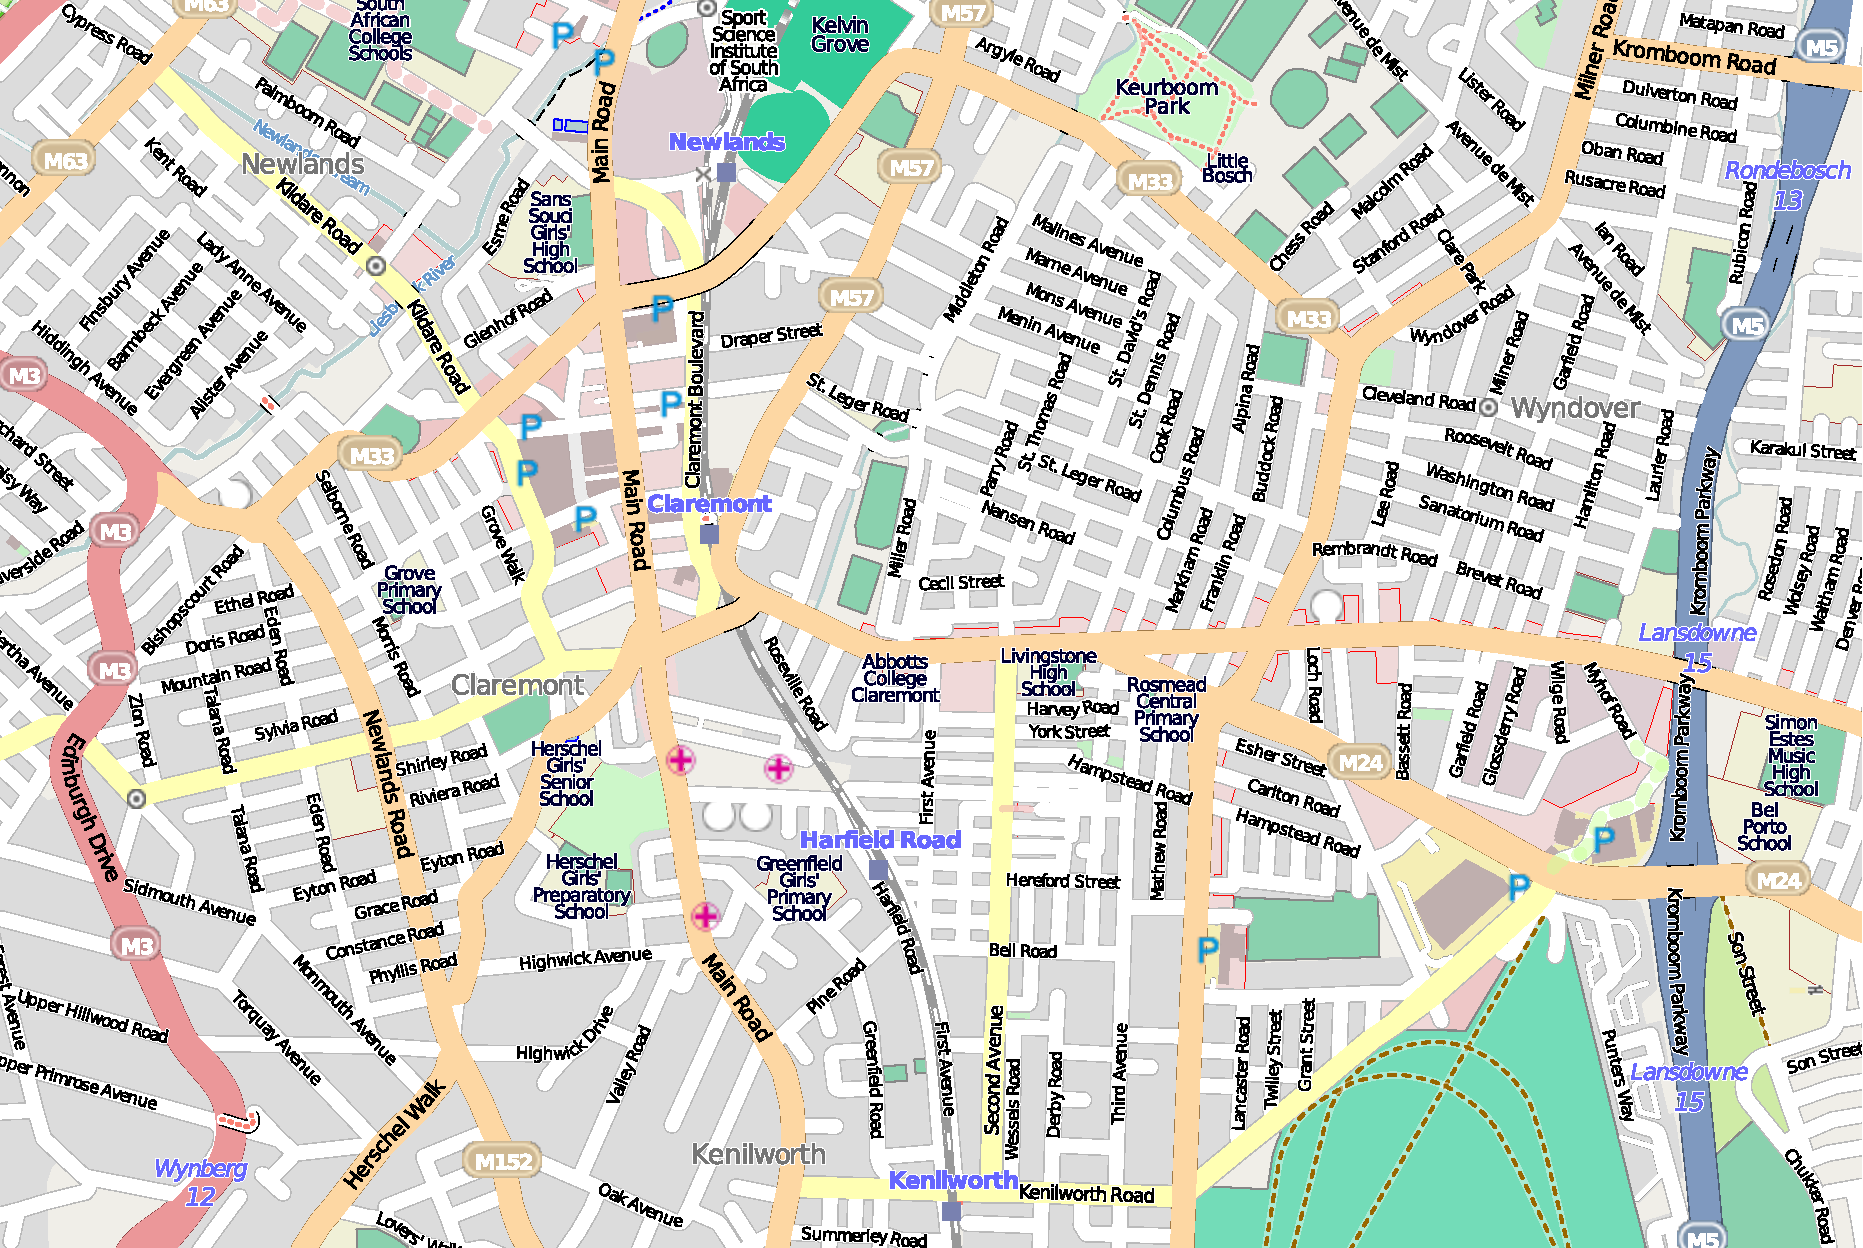
\includegraphics[width=0.25\linewidth]{context/vector_map}
	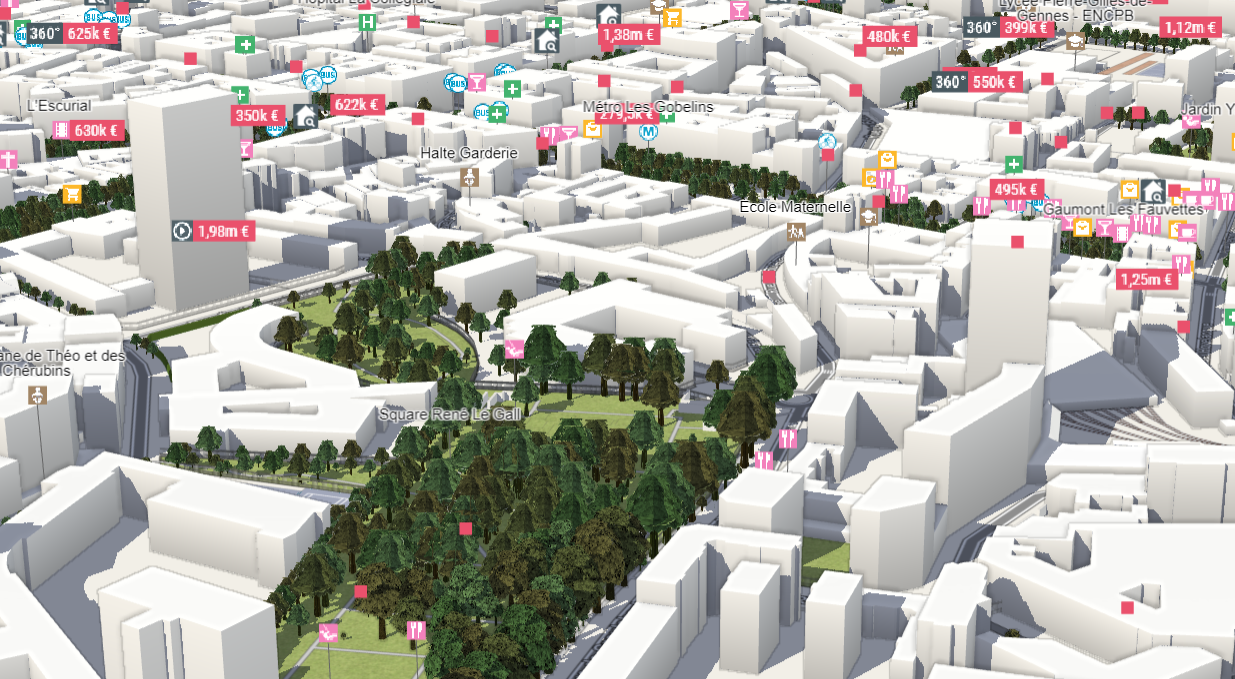
\includegraphics[width=0.25\linewidth]{context/lod_visu}
	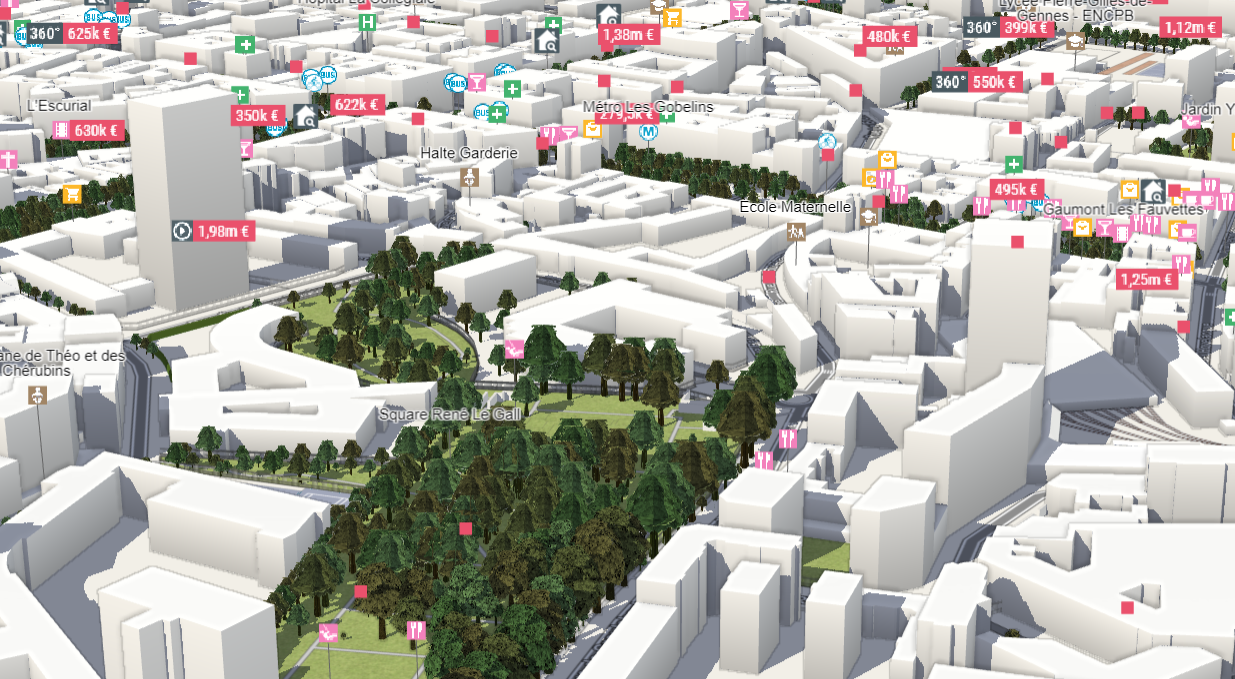
\includegraphics[width=0.25\linewidth]{context/lod_visu}
\end{frame}

\begin{frame}{Why do we need 3D models?}
	\begin{itemize}
		\item\uncover<1->{Visualization}
		\item\uncover<2->{Simulation}
		\item\uncover<3->{Change tracking}
	\end{itemize}
	
	\begin{minipage}[t][0.2\textheight][r]{\linewidth}
		\centering
		\only<1>{
			\begin{figure}
				\centering
				\begin{subfigure}[t]{0.45\linewidth}
					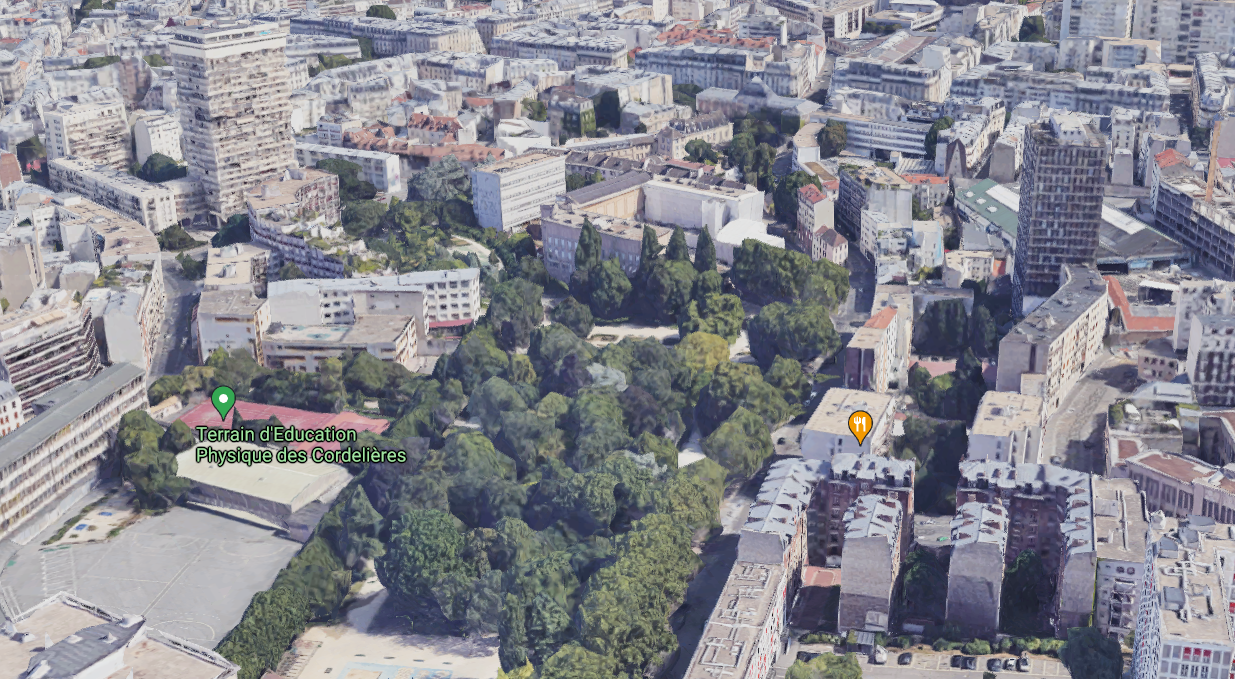
\includegraphics[width=\linewidth]{context/dense_visu}
					\subcaption*{Dense mesh representation \footnote[frame]{Google Maps}}
				\end{subfigure}
				\begin{subfigure}[t]{0.45\linewidth}
					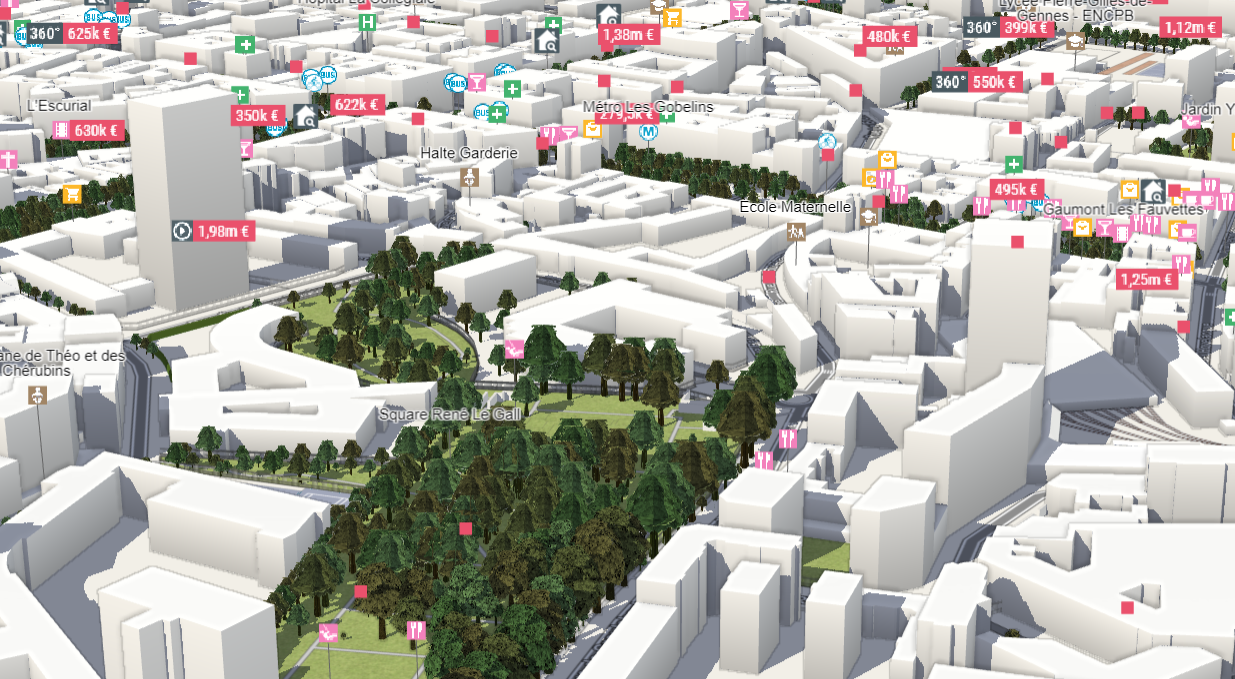
\includegraphics[width=\linewidth]{context/lod_visu}
					\subcaption*{LOD1 visualization \footnote[frame]{Bien'ici}}
				\end{subfigure}
			\end{figure}
		}
		
		\only<2>{
			\begin{figure}
				\begin{subfigure}[t]{0.45\linewidth}
					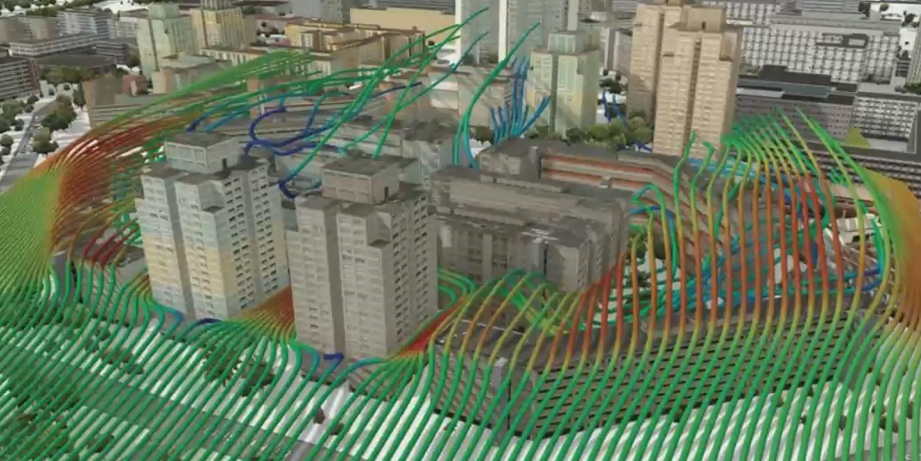
\includegraphics[width=\linewidth]{context/simulation_wind}
					\subcaption*{Wind simulation \footnote[frame]{SIMULIA, Dassault Systèmes}}
				\end{subfigure}
				\begin{subfigure}[t]{0.45\linewidth}
					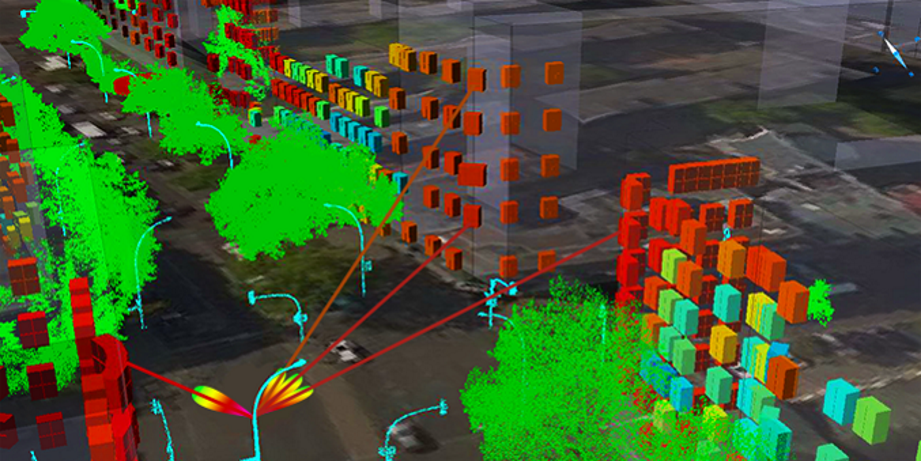
\includegraphics[width=\linewidth]{context/simulation_lineofsight}
					\subcaption*{5G connectivity simulation \footnote[frame]{SIRADEL}}
				\end{subfigure}
			\end{figure}
		}
		
		\only<3>{}
	\end{minipage}
\end{frame}

\begin{frame}{Acquisitions}			
	Existing GIS data (incorrect)
	LiDAR technologies
	Imagery (airborne or drone) -> Photogrammetry
	
\end{frame}

\begin{frame}{Scope of interest}
	Point clouds either LiDAR or photogrammetry. \\
	Semi-automatic  \\
	Large-scale parsimonious representation \\
	Small-scale dense representation
\end{frame}